\documentclass[a4paper,12pt]{article}
\usepackage{graphicx}
\usepackage{fancyhdr}


\pagestyle{fancy}
\lhead{Algorithms and Data Structure 8}
\rhead{Drishti Maharjan}

\begin{document}
\title{Algorithms and Data Structures }
\author{Drishti Maharjan}
\maketitle

\section*{\center Assignment 8}

\subsection*{\newpage Problem 8.1 \newline}
\subsubsection*{\textnormal { a. Insertion in the order [13; 44; 37; 7; 22; 16]: \newline \newline
\textit{Note: Visualization website was used to get the images of trees and the colors and screenshots of steps have been pasted} \newline
\begin{figure}[h!]
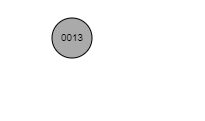
\includegraphics{1a1.png}
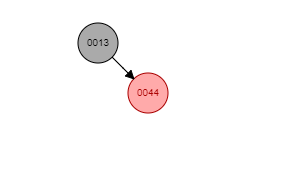
\includegraphics{1a2_1.png}
\caption{Inserting 13 and 44}
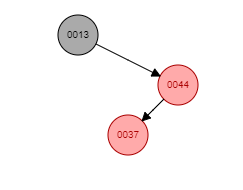
\includegraphics{1a3_1.png}
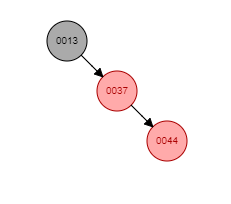
\includegraphics{1a3_2.png}
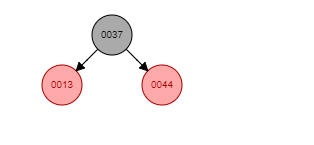
\includegraphics{1a3_3.png}
\caption {Inserting 37}
\end{figure}
\newpage
\begin{figure} [h!]
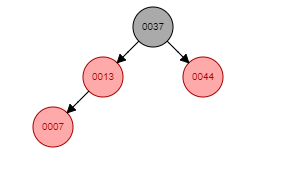
\includegraphics{1a4_1.png}
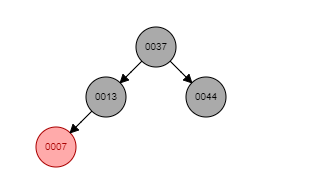
\includegraphics{1a4_2.png}
\caption{Inserting 7}
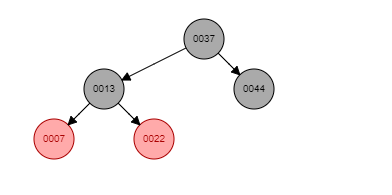
\includegraphics{1a5_1.png}
\caption{Inserting 22}
\end{figure}
\begin{figure} [h!]
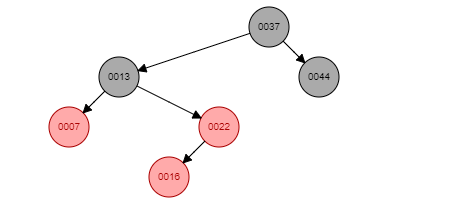
\includegraphics{1a6_1.png}
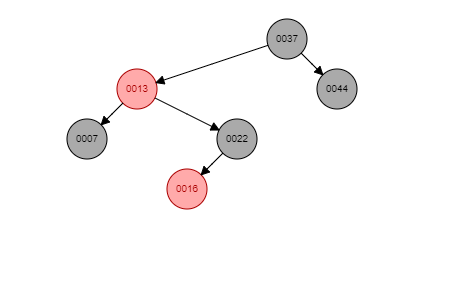
\includegraphics{1a6_2.png}
\caption{Inserting 16}
\end{figure} }}
\newpage 
\subsubsection*{\textnormal { \newline \newline \newline \newline b. All permutations of [1,2,3,4] were taken and red black tree was implmented with the help of C++ implementation for problem 8.2 and lecture notes. All nil nodes are black leaves, which are not shown in the trees here. And, possible 4 trees are drawn below: \newline 
\begin{figure} [h!]
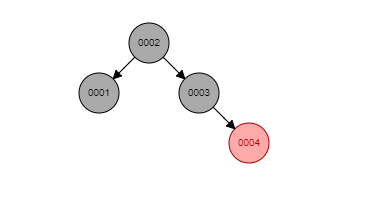
\includegraphics{1b1.png}
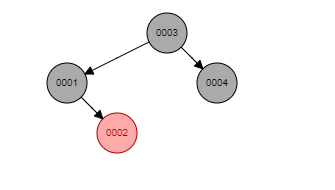
\includegraphics{1b2.png}
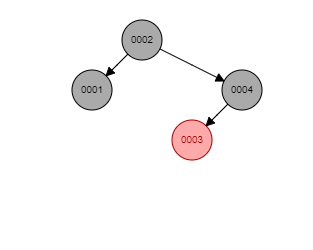
\includegraphics{1b3.png}
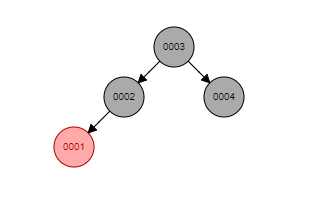
\includegraphics{1b4.png}
\end{figure} }}

\newpage

\subsubsection*{\textnormal { \newpage c. \textbf {Proof by Induction} \newline \newline
\textit {Base Case:}
\newline 
N = 2. The node to be inserted is red and root is black by default, and no properties are violated so no fixup is required. No of red node = 1.
\newline \newline
\textit {Inductive Hypothesis:} Let's suppose that for a red black tree of n nodes, there exists at least 1 red node for $ 1 < n <= N $.
\newline \newline \textit{Inductive Step:} We need to prove that for a red black tree of $N+1$ nodes, there exists at least 1 red node.
\newline \newline
While inserting the $ N+1$ element, we will have to consider 2 cases:
\newline \newline
Case 1 :  The inserted Red Node is a child of a black node. This is also equivalent to the base case, which has been proved already.
\newline \newline
Case 2: Red Node $N+1$ is inserted as a child of a red node. This violates the property of Red Black Tree, so we need to fix it to balance the tree.
Let's look at the insertion cases that have X as a child of a red node P. This divides into further cases: [P-parent, G-grandparent, U-uncle] \newline \newline 
Insertion Case 1: P,G,U is recolored and X remains red after the recoloring. It stil retains the
same color after we move reference X to Grandparent of X. Thus, this remains a red node, giving us at least 1 red node.
\newline \newline
Insertion Case 2: X is rotated about P and then G, this retains the red color of parent P. X and G is recolored while color of P remains the same i.e. Red. So,we have at least one red node.
\newline \newline
Insertion Case 3: X remains red after the rotation of P about G. X remains red after
the recoloring of P and G. Thus we have atleast 1 red node.
\newline \newline 
Hence, the claim has been proved. \newline \newline}}

\subsection*{Problem 8.2\newline}
\subsubsection*{\textnormal{a. Code in testRBT.cpp and redblacktree.h, and Makefile in Makefile.txt}}


\end{document}
